\section{Numerical Integration and Solution of Ordinatry Diffential Equations}


\subsection{Problem 7.12}


\begin{figure}[!ht]
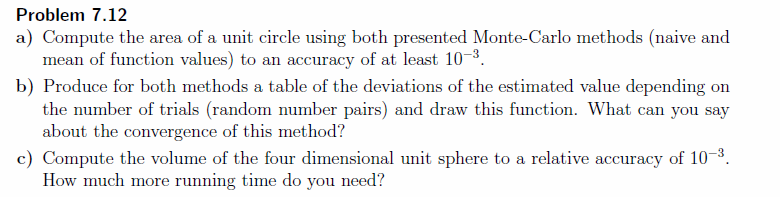
\includegraphics[width=1\textwidth]{chapters/images/desc-7-12}
\end{figure}


\subsubsection{a)}

First we need a function whose integral over a certain interval is equal the area of the unit circle. The integral of the function $\sqrt{1 - x^2}$ over the interval $[-1, 1]$ equals half the area of the unit circle, so with a little tweaking of the parameter $x$ we can modify the function to have an integral equal to the unit circle over the interval $[0, 4]$. The function in Python looks the following way:

\begin{lstlisting}[caption=Function for the unit circle area]
def circleF(x):
	newX = (x % 2) - 1;
	return math.sqrt(1 - pow(newX, 2));
\end{lstlisting}

Afterwards, we can use this function for the calculation of the area with both the naive and mean Monte Carlo method:

\begin{lstlisting}[caption=Problem 7.12 a)]
goal = math.pi;

def getRandCoord(a, b):
	return random.random() * (b - a) + a;

def doNaiveMonteCarloTest(xMin, xMax, yMin, yMax):
	randX = getRandCoord(xMin, xMax);
	randY = getRandCoord(yMin, yMax);
	
	return circleF(randX) > randY;

def doNaiveMonteCarlo(precision):
	areaEstimated = 0;
	tries = 0.0;
	successes = 0.0;

	while abs(areaEstimated - goal) > precision:
		if doNaiveMonteCarloTest(0, 4, 0, 1):
			successes += 1;
		
		tries += 1;
		
		areaEstimated = 4 * (successes / tries);
	
	return [areaEstimated, tries];

def doMeanMonteCarlo(precision):
	areaEstimated = 0;
	tries = 0.0;
	sum = 0.0;
	
	while abs(areaEstimated - goal) > precision:
		randX = getRandCoord(0, 4);
		
		sum += circleF(randX);
		tries += 1;
		
		areaEstimated = 4 * (sum / tries);
	
	return [areaEstimated, tries];

minError = 0.001;

naiveMonteCarlo = doNaiveMonteCarlo(minError);
print("naive method:");
print("estimated area: " + str(naiveMonteCarlo[0]));
print("tries: " + str(naiveMonteCarlo[1]));

meanMonteCarlo = doMeanMonteCarlo(minError);
print("mean value method:");
print("estimated area: " + str(meanMonteCarlo[0]));
print("tries: " + str(meanMonteCarlo[1]));
\end{lstlisting}

The results of those calculations are:

\begin{lstlisting}[caption=Result of 7.12 a), keywordstyle=\color{black}]
naive method:
estimated area: 3.14241702843
tries: 7141.0

mean value method:
estimated area: 3.14239623321
tries: 658.0
\end{lstlisting}


\subsubsection{b)}

To calculate the deviation we can use a slightly alternative version of the Monte Carlo functions of a).

\begin{lstlisting}[caption=Problem 7.13 b)]
def getNaiveMonteCarloDeviation(tries):
	successes = 0.0;
	
	for i in range(tries):
		if doNaiveMonteCarloTest(0, 4, 0, 1):
			successes += 1;
	
	areaEstimated = 4 * (successes / tries);
	
	return abs(areaEstimated - goal);

def getMeanMonteCarloDeviation(tries):
	sum = 0.0;
	
	for i in range(tries):
		randX = getRandCoord(0, 4);
		
		sum += circleF(randX);
	
	areaEstimated = 4 * (sum / tries);
	
	return abs(areaEstimated - goal);

xses = [];
naiveYses = [];
meanYses = [];

for i in range(1, 250):
	naiveDeviation = getNaiveMonteCarloDeviation(i * 10);
	meanDeviation = getMeanMonteCarloDeviation(i * 10);
	
	xses.append(i);
	naiveYses.append(naiveDeviation);
	meanYses.append(meanDeviation);

plt.plot(xses, naiveYses);
plt.plot(xses, meanYses);
plt.xlabel("tries");
plt.ylabel("deviation");
plt.show();
\end{lstlisting}

\newpage

The resulting graph looks like this:

\begin{figure}[!ht]
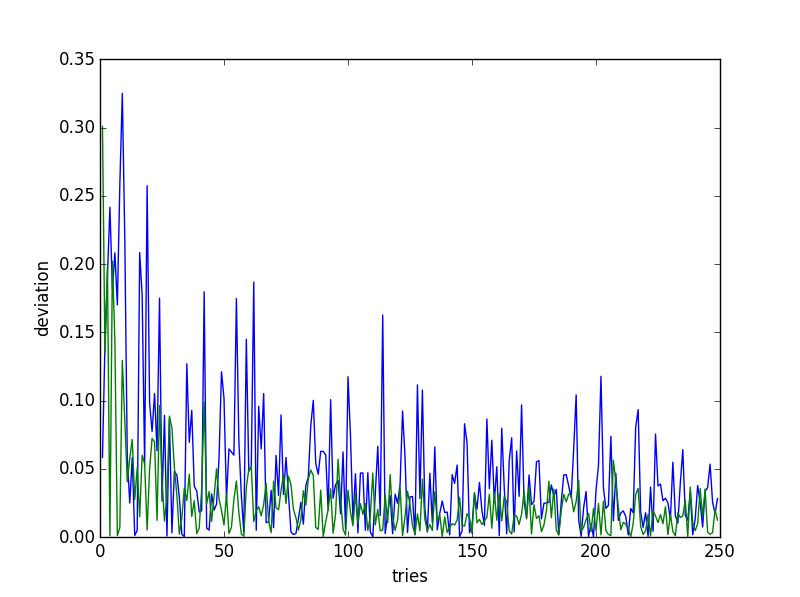
\includegraphics[width=1\textwidth]{chapters/images/figure-7-12-b}
\caption{Deviation of the Monte Carlo methods}
\end{figure}

Although the deviation tends to get smaller and smaller there is no convergence. Due to the random factor both functions have there is no guarantee the $y$ values get close to a certain value.


\subsubsection{c)}

To calculate the volume we again need a function to check whether a random point is within our body of choice. For an n-dimensional unit sphere we can simply check whether the length of the n-dimensional vector of the coordinates is shorter than 1. If so, the point is within the sphere. The Python function for the four-dimensional sphere can be implemented in the following way:

\begin{lstlisting}[caption=Function for the 4D unit sphere volume]
def isIn4DSphere4D(x, y, z, a):
	return math.sqrt(pow(x, 2) + pow(y, 2) + pow(z, 2) + pow(a, 2)) < 1;
\end{lstlisting}

Again we use this function for the Monte Carlo method to calculate the volume the same way we did in the subtask a):

\begin{lstlisting}[caption=4D unit sphere volume calculation]
def doNaiveMonteCarloTest4D():
	randX = getRandCoord(0, 1);
	randY = getRandCoord(0, 1);
	randZ = getRandCoord(0, 1);
	randA = getRandCoord(0, 1);
	
	return isIn4DSphere4D(randX, randY, randZ, randA);

goal2 = pow(math.pi, 2) / 2.0;

def doNaiveMonteCarlo4D(precision):
	areaEstimated = 0;
	tries = 0.0;
	successes = 0.0;

	while abs(areaEstimated - goal2) > precision:
		if doNaiveMonteCarloTest4D():
			successes += 1;
		
		tries += 1;
		
		areaEstimated = 16 * (successes / tries);
	
	return [areaEstimated, tries];

fourDSphere = doNaiveMonteCarlo4D(minError);
print("estimated area of 4D unit sphere: " + str(fourDSphere[0]));
\end{lstlisting}

The result of the calculation is the following:

\begin{lstlisting}[caption=Result of the 4D unit sphere volume calculation, keywordstyle=\color{black}]
estimated area of 4D unit sphere: 4.93493975904
\end{lstlisting}

Afterwards we can analyze the computational time of both methods:

\begin{lstlisting}[caption=Problem 7.12 c)]
total2DTries = 0.0;
total4DTries = 0.0;

runs = 250;

for i in range(runs):
	total2DTries += doNaiveMonteCarlo(minError)[1];
	total4DTries += doNaiveMonteCarlo4D(minError)[1];

avg2DTries = total2DTries / float(runs);
avg4DTries = total4DTries / float(runs);

print("average tries for 2d unit circle: " + str(avg2DTries));
print("average tries for 4d unit sphere: " + str(avg4DTries));
\end{lstlisting}

The results of these calculations are:

\begin{lstlisting}[caption=Result of 7.12 c), keywordstyle=\color{black}]
average tries for 2d unit circle: 4928.92
average tries for 4d unit sphere: 14141.112
\end{lstlisting}

Looking at the results, it takes about 3 times as much computational time to calculate the volume of a 4 dimensional unit sphere than it is to calculate the area of a 2 dimensional unit circle.


\subsection{Problem 7.13}


\begin{figure}[!ht]
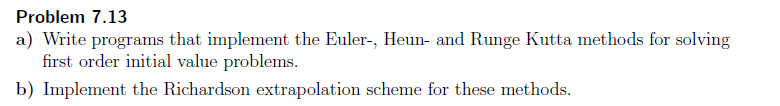
\includegraphics[width=1\textwidth]{chapters/images/desc-7-13}
\end{figure}


\subsubsection{a)}

To solve an ODE, first a general function can be defined for the basic approach. To make this function applicable for different approximation methods (like Euler method and Runge-Kutta method) the function which defines how to calculate the $y_{n + 1}$ value will be passed as an argument. This abstract function will be called \textit{yp1Method} in this exercise.

\begin{lstlisting}[caption=Function to solve ODE]
def odeSolver(f, a, b, y0, h, yp1Method):
	x = a;
	y = y0;
	
	yses = [];
	yses.append(y);
	
	while x <= b:
		y = yp1Method(f, x, y, h);
		yses.append(y);
		
		x += h;
	
	return yses;
\end{lstlisting}

Afterwards, we need to define the \textit{yp1Method} functions for the Euler, Heun, and Runge-Kutta methods.

\begin{lstlisting}[caption=YP1Methods]
def eulerYP1(f, x, y, h):
	return y + h * f(x, y);

def heunYP1(f, x, y, h):
	k1 = h * f(x, y);
	k2 = h * f(x + h, y + k1);
	
	return y + 0.5 * (k1 + k2);

def rungeKuttaYP1(f, x, y, h):
	k1 = h * f(x, y);
	k2 = h * f(x + 0.5 * h, y + 0.5 * k1);
	k3 = h * f(x + 0.5 * h, y + 0.5 * k2);
	k4 = h * f(x + h, y + k3);
	
	return y + (1 / 6.0) * (k1 + 2 * k2 + 2 * k3 + k4);
\end{lstlisting}

The final ODE solving functions for each method can now call the basic \textit{odeSolver} function and pass the respective \textit{yp1Method}:

\begin{lstlisting}[caption=ODE solving functions for each method]
def euler(f, a, b, y0, h):
	return odeSolver(f, a, b, y0, h, eulerYP1);

def heun(f, a, b, y0, h):
	return odeSolver(f, a, b, y0, h, heunYP1);

def rungeKutta(f, a, b, y0, h):
	return odeSolver(f, a, b, y0, h, rungeKuttaYP1);
\end{lstlisting}

To solve an ODE system the function has to be altered a little bit.

\begin{lstlisting}[caption=Function to solve an ODE system]
def odeSystemSolver(fVector, a, b, y0Vector, h, yp1Methods):
	yVectorses = [];
	
	x = a;
	yVector = y0Vector;
	
	yVectorses.append(yVector);
	
	while x <= b:
		yp1Vector = yp1Methods(fVector, x, yVector, h);
		
		yVectorses.append(yp1Vector);
		
		yVector = yp1Vector;
		
		x += h;
	
	return yVectorses;
\end{lstlisting}

Also a new \textit{yp1Method} has to be defined:

\begin{lstlisting}[caption=YP1Method for solving an ODE system]
def rungeKuttaYP1System(fVector, x, yVector, h):
	nF = len(fVector);
	
	k1Vector = [];
	yVectorPlusHalfK1Vector = [];
	
	for i in range(nF):
		k1El = h * fVector[i](x, yVector);
		k1Vector.append(k1El);
		yVectorPlusHalfK1Vector.append(yVector[i] + 0.5 * k1El);
	
	k2Vector = [];
	yVectorPlusHalfK2Vector = [];
	
	for i in range(nF):
		k2El = h * fVector[i](x + 0.5 * h, yVectorPlusHalfK1Vector);
		k2Vector.append(k2El);
		yVectorPlusHalfK2Vector.append(yVector[i] + 0.5 * k2El);
	
	k3Vector = [];
	yVectorPlusK3Vector = [];
	
	for i in range(nF):
		k3El = h * fVector[i](x + 0.5 * h, yVectorPlusHalfK2Vector);
		k3Vector.append(k3El);
		yVectorPlusK3Vector.append(yVector[i] + k3El);
	
	yp1Vector = [];
	
	for i in range(nF):
		k4El = h * fVector[i](x + h, yVectorPlusK3Vector);
		
		yp1 = yVector[i] + (1 / 6.0) * (k1Vector[i] + 2 * k2Vector[i] + 2 * k3Vector[i] + k4El);
		
		yp1Vector.append(yp1);
	
	return yp1Vector;

def rungeKuttaSystem(fVector, a, b, y0Vector, h):
	return odeSystemSolver(fVector, a, b, y0Vector, h, rungeKuttaYP1System);
\end{lstlisting}


\subsubsection{b)}

For the Richardson extrapolation we need to define new functions for the different \textit{yp1Methods} again to calculate the value of the next $y$ value. However, the basic ODE solving function can be reused.

\begin{lstlisting}[caption=Problem 7.13 b)]
def fkFunc(f, x, y, h, yp1Func, q, pk, step):
	if step == 1:
		fh = yp1Func(f, x, y, h);
		fqh = yp1Func(f, x, y, q * h);
	else:
		fh = fkFunc(f, x, y, h, yp1Func, q, pk, step - 1);
		fqh = fkFunc(f, x, y, q * h, yp1Func, q, pk, step - 1);
	
	return fh + ((fh - fqh) / (pow(q, pk) - 1.0));

def eulerYP1Richardson(f, x, y, h):
	return fkFunc(f, x, y, h, eulerYP1, 5, 23, 5);

def heunYP1Richardson(f, x, y, h):
	return fkFunc(f, x, y, h, heunYP1, 2, 13, 5);

def rungeKuttaYP1Richardson(f, x, y, h):
	return fkFunc(f, x, y, h, rungeKuttaYP1, 4, 18, 5);

def eulerRichardson(f, a, b, y0, h):
	return odeSolver(f, a, b, y0, h, eulerYP1Richardson);

def heunRichardson(f, a, b, y0, h):
	return odeSolver(f, a, b, y0, h, heunYP1Richardson);

def rungeKuttaRichardson(f, a, b, y0, h):
	return odeSolver(f, a, b, y0, h, rungeKuttaYP1Richardson);
\end{lstlisting}

The required values for $q$ and $p_{k}$ have been empirically determined for each method.


\subsection{Problem 7.14}

%\begin{figure}[!ht]
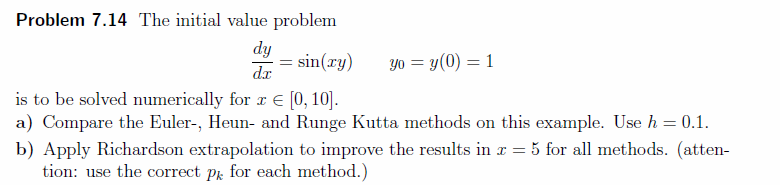
\includegraphics[width=1\textwidth]{chapters/images/desc-7-14}
%\end{figure}


\subsubsection{a)}

To calculate the respective $y$ values we can simply use the functions from Problem 7.13:

\begin{lstlisting}[caption=Problem 7.14 a)]
def myF(x, y):
	return math.sin(x * y);

xses = [];

for i in range(102): xses.append(i / 10.0);

eulerYses = dif.euler(myF, 0, 10, 1, 0.1);
heunYses = dif.heun(myF, 0, 10, 1, 0.1);
rungeKuttaYses = dif.rungeKutta(myF, 0, 10, 1, 0.1);

plt.plot(xses, eulerYses);
plt.plot(xses, heunYses);
plt.plot(xses, rungeKuttaYses);
plt.xlabel("x");
plt.ylabel("y");
plt.show();
\end{lstlisting}

The resulting graph of each method looks like the following:

\newpage

\begin{figure}[!ht]
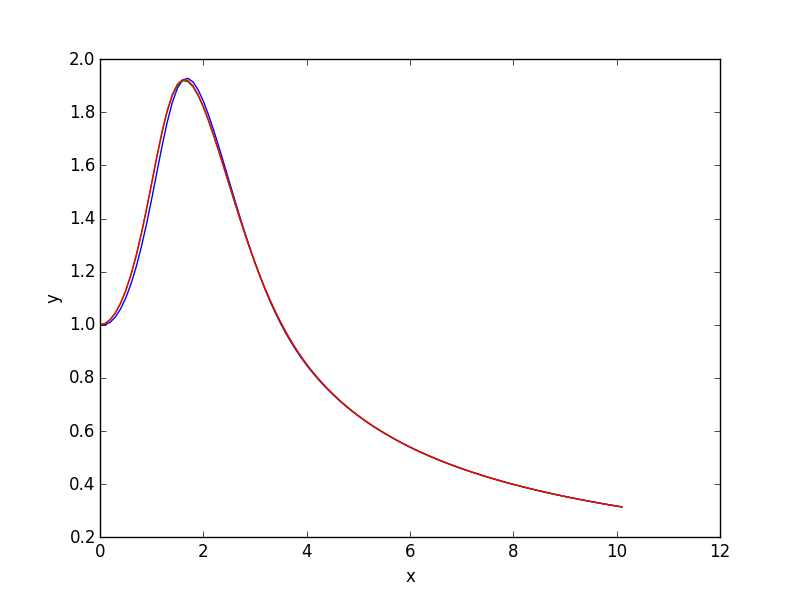
\includegraphics[width=1\textwidth]{chapters/images/figure-7-14-a}
\caption{Graph of the results of the 3 methods}
\end{figure}

As it can be seen, the graphs of the functions are very close to each other and there is hardly any difference noticeable.

\subsubsection{b)}

Again, using the functions from Problem 7.13 we can simply calculate the $y$ values with the Richardson extrapolation:

\begin{lstlisting}[caption=Problem 7.14 b)]
eulerRichardsonYses = dif.eulerRichardson(myF, 0, 10, 1, 0.1);
heunRichardsonYses = dif.heunRichardson(myF, 0, 10, 1, 0.1);
rungeKuttaRichardsonYses = dif.rungeKuttaRichardson(myF, 0, 10, 1, 0.1);

print("euler: " + str(eulerRichardsonYses[50]));
print("heun: " + str(heunRichardsonYses[50]));
print("runge-kutta: " + str(rungeKuttaRichardsonYses[50]));
\end{lstlisting}

The result of these calculations are:

\begin{lstlisting}[caption=Result of 7.14 b), keywordstyle=\color{black}]
euler: 0.656662162824
heun: 0.657837825456
runge-kutta: 0.657541150858
\end{lstlisting}

As expected, the value approximated with Euler's method is slightly below the other method's values, however with the Richardson extrapolation this error is not as critical as it would have been if the regular methods had been used.


\subsection{Problem 7.15}


\begin{figure}[!ht]
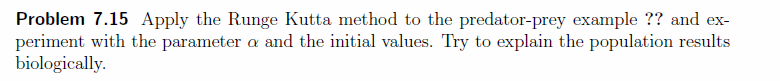
\includegraphics[width=1\textwidth]{chapters/images/desc-7-15}
\end{figure}

To simulate the predator-prey-model an ODE system has to be created, with one equation for the sheep and one for the wolfs. Afterwards, the solution can be simply calculated with the script from Problem 7.13:

\begin{lstlisting}[caption=Problem 7.15]
def sheepFunc(t, yVector):
	return 10 * yVector[0] * (1 - yVector[1]);

def wolfsFunc(t, yVector):
	return yVector[1] * (yVector[0] - 1);

fses = [];
y0ses = [];

fses.append(sheepFunc);
fses.append(wolfsFunc);
y0ses.append(3);
y0ses.append(1);

yVectors = dif.rungeKuttaSystem(fses, 0, 5, y0ses, 0.05);

xses = [];
sheepYses = [];
wolfsYses = [];

x = 0;

for yVector in yVectors:
	sheepYses.append(yVector[0]);
	wolfsYses.append(yVector[1]);
	xses.append(x);
	x += 0.05;

plt.plot(xses, sheepYses);
plt.plot(xses, wolfsYses);
plt.xlabel("x");
plt.ylabel("y");
plt.show();
\end{lstlisting}

Depending on $\alpha$ and the initial number of sheep and wolfs the graphs look like this:

\begin{figure}[!ht]
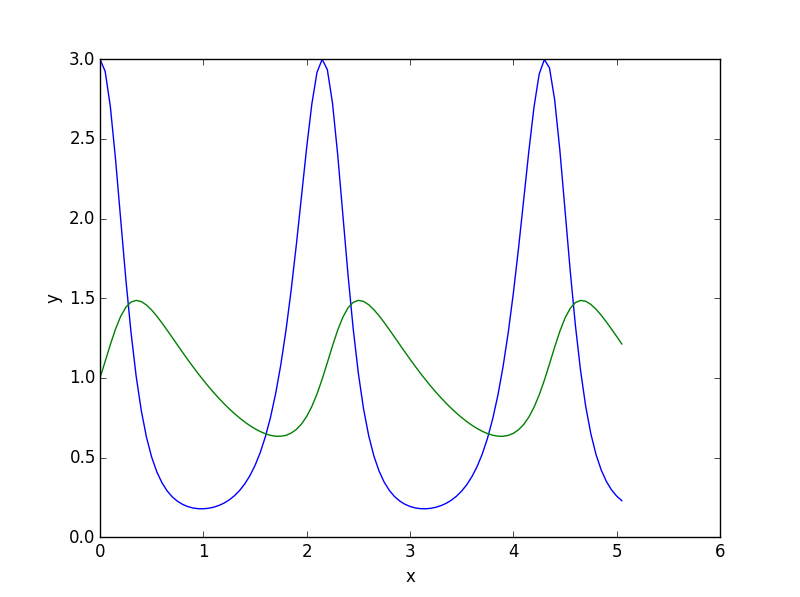
\includegraphics[width=1\textwidth]{chapters/images/figure-7-15-1}
\caption{$\alpha = 10$, initially 3 sheep and 1 wolfs}
\end{figure}

\begin{figure}[!ht]
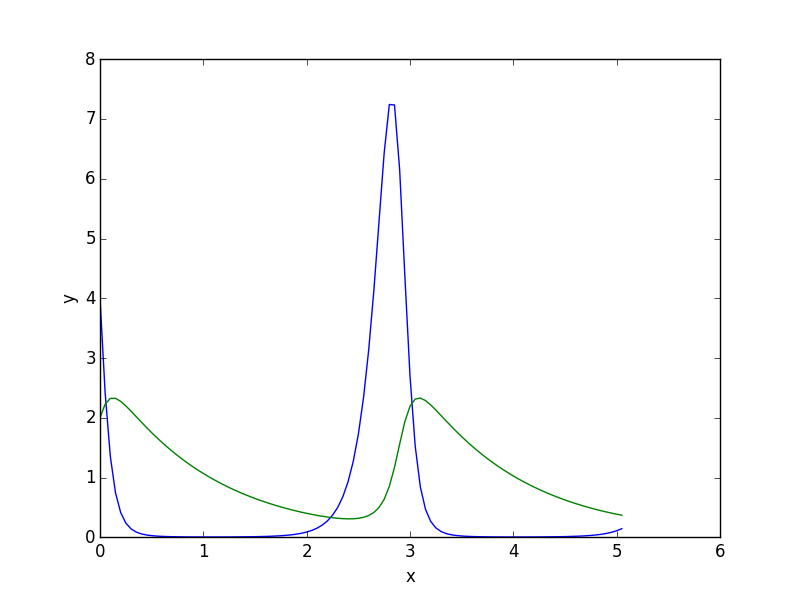
\includegraphics[width=1\textwidth]{chapters/images/figure-7-15-2}
\caption{$\alpha = 9$, initially 4 sheep and 2 wolfs}
\end{figure}

\begin{figure}[!ht]
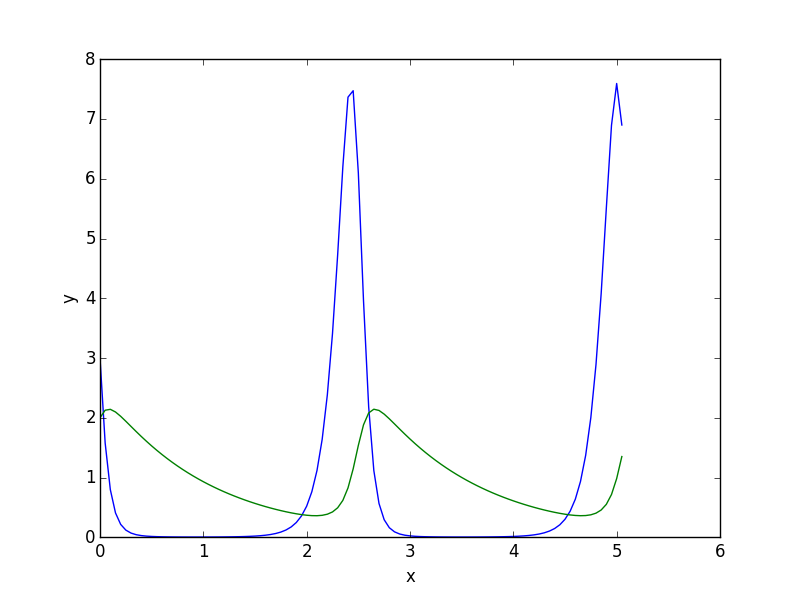
\includegraphics[width=1\textwidth]{chapters/images/figure-7-15-3}
\caption{$\alpha = 12$, initially 3 sheep and 2 wolfs}
\end{figure}

Biologically, this could be explained by the balance between predator and prey which is mandatory for both species to survive.


\newpage

\subsection{Problem 7.16}

\begin{figure}[!ht]
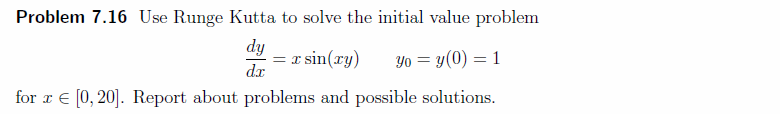
\includegraphics[width=1\textwidth]{chapters/images/desc-7-16}
\end{figure}

\begin{lstlisting}[caption=Problem 7.16]
def myF(x, y):
	return x * math.sin(x * y);

xses = [];

for i in range(201): xses.append(i / 10.0);

yses = dif.rungeKutta(myF, 0, 20, 1, 0.1);

plt.plot(xses, yses);
plt.xlabel("x");
plt.ylabel("y");
plt.show();
\end{lstlisting}

The resulting graph looks like:

\begin{figure}[!ht]
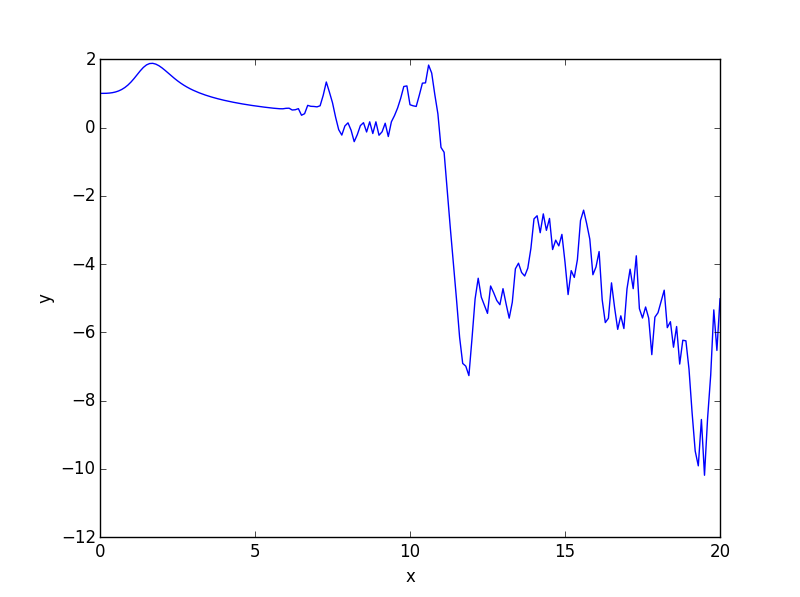
\includegraphics[width=1\textwidth]{chapters/images/figure-7-16}
\caption{Graph of Problem 7.16}
\end{figure}


Since the $x$ parameter is a factor both inside and outside of the sine, the frequency as well as the amplitude increase as $x$ grows. Hence, the fluctuation increases and the slopes get steeper and steeper. Because the step size stays the same, the curve gets \enquote{spikier} and slightly inaccurate. A possible solution could be to decrease the step size.

